\newpage
\subsection{The sensors}
\begin{figure}[!h]
    \centering
    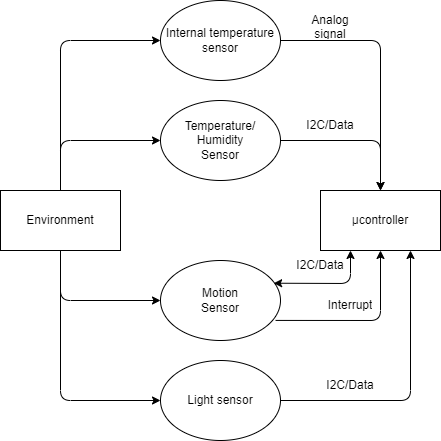
\includegraphics[width=0.8\textwidth]{\currfiledir/figures/sensor_diagram.png}
    \caption{Architecture diagram of the sensors and their relationship to other components}
\end{figure}

\noindent Our aim was to ultimately add sensors to the system in order to send information about it with the LoRa communication protocol. The researchers can then know the state of the system in real time, in order to not lose days or even weeks of pictures collected if the system has a problem.\\
In fact, the environment could perturbate the environment in 2 different ways:\\
The system could move (because of wind or potentially animals), which would unbalance the system. The system could then fall on the ground or take pictures of the wrong place. The researchers not knowing it could let the system in place during months, which could lead to a loss of time in their work.\\
The system could also be damaged by bad weather conditions, such as humidity and temperature. For example, if the temperature rises too much, the battery and other components could be damaged. So, it is important to detect the problems to inform the researchers.\\
The sensors would collect data in the environment and send it to the microcontroller in order to process it and log it. Then, the data would be sent to the storage system.




\newpage
\subsubsection{Motion sensor}
The motion sensor employed in this device is an ICM-20602. This motion tracking device was chosen for its low power consumption (1.33mA in low power mode and 2.79mA when in low noise mode). The ICM-20602 is also programmable, allowing users to define a threshold value to wake up the microcontroller.
For communication, the ICM-20602 utilizes an I2C interface, as well as an interrupt pin to signal events such as data-ready or wake-on-motion. This makes it easy to interface with a microcontroller and manage the sensor's operation.
The output data rate (ODR) for both the accelerometer and gyroscope can be configured based on your application requirements. When using interrupt-driven data collection, the interrupt pin can be set to trigger when new data is available, allowing the microcontroller to process the information.

\begin{figure}[!h]
    \centering
    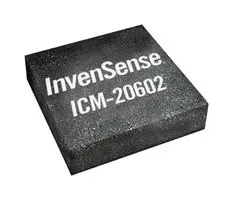
\includegraphics[width=0.4\textwidth]{\currfiledir/figures/20602.png}
    \caption{Picture of the motion sensor ICM-20602}
    \cite{20602}
\end{figure}

\newpage
\subsubsection{Humidity/Temperature sensor}
The AM2320 has been selected as the humidity and temperature sensor for this project due to its affordability and low power consumption (maximum 1mA and 50µA in sleep mode). This sensor covers a wide temperature range from -40 to 80°C and is capable of measuring humidity from 0 to 99.9\% relative humidity. The AM2320 is also equipped with an I2C connection, making it convenient for integration with a microcontroller.
In this application, humidity and temperature will be measured every 30 minutes. The I2C interface of the AM2320 facilitates communication with the microcontroller, allowing for efficient and accurate data collection at regular intervals. This ensures that the project remains energy-efficient while providing reliable temperature and humidity measurements.

%: Picture of the temperature and humidity sensor AM2320.
\begin{figure}[!h]
    \centering
    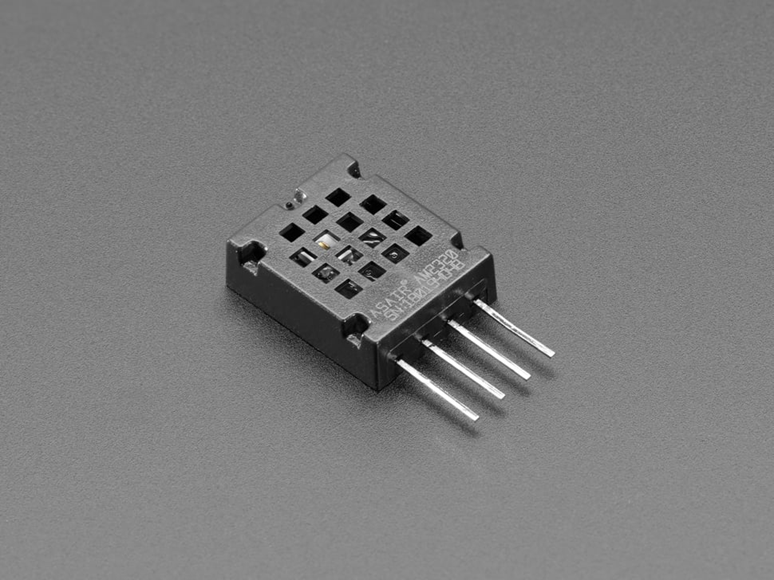
\includegraphics[width=0.4\textwidth]{\currfiledir/figures/AM2320.png}
    \caption{Picture of the temperature and humidity sensor AM2320}
    \cite{AM2320}
\end{figure}


\subsubsection{Temperature sensors}
The LM35DZ temperature sensor is selected for internal case temperature monitoring due to its high accuracy, low power consumption (less than 60µA), and easy interfacing with a microcontroller. It provides a linear output (10mV/°C), operates in a -55 to 150°C range, and minimizes self-heating, which reduces measurement interference. Temperature measurements will be taken every 30 minutes, ensuring energy-efficient and reliable monitoring.
\begin{figure}[!h]
    \centering
    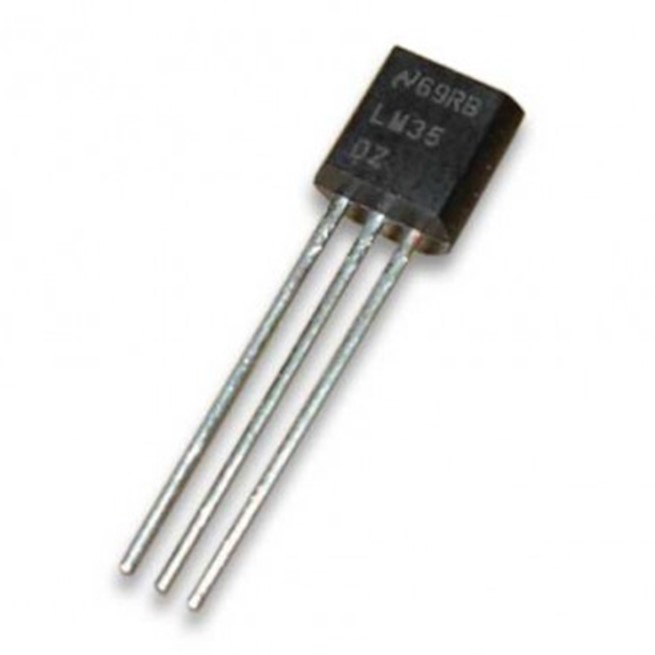
\includegraphics[width=0.25\textwidth]{\currfiledir/figures/LM35DZ.jpg}
    \caption{Temperature sensors LM35DZ}
    \cite{Temp}
\end{figure}



\newpage
\subsubsection{Light sensor}
For light sensing requirements, the chosen sensor is the TSL2561. This efficient and cost-effective sensor is known for its reliable light intensity measurements across a wide range of conditions. One of the key reasons for selecting the TSL2561 is its low power consumption, with a typical active current of 0.24mA and a power-down current of 2µA, which aligns with the project's focus on energy efficiency. Additionally, the sensor boasts a range of 0.1 to 40,000 lux, making it suitable for various lighting environments. The availability of the TSL2561 for quick delivery further contributed to this decision. Its I2C interface enables integration with the microcontroller, while the high-resolution 16-bit digital output ensures accurate and precise light readings.
In this application, the TSL2561 operates with an I2C interface and takes light measurements every 30 minutes. Additionally, a measurement is taken before capturing a photo to ensure optimal lighting conditions. This approach guarantees energy-efficient and precise light readings, contributing to the overall effectiveness of the project.
\begin{figure}[!h]
    \centering
    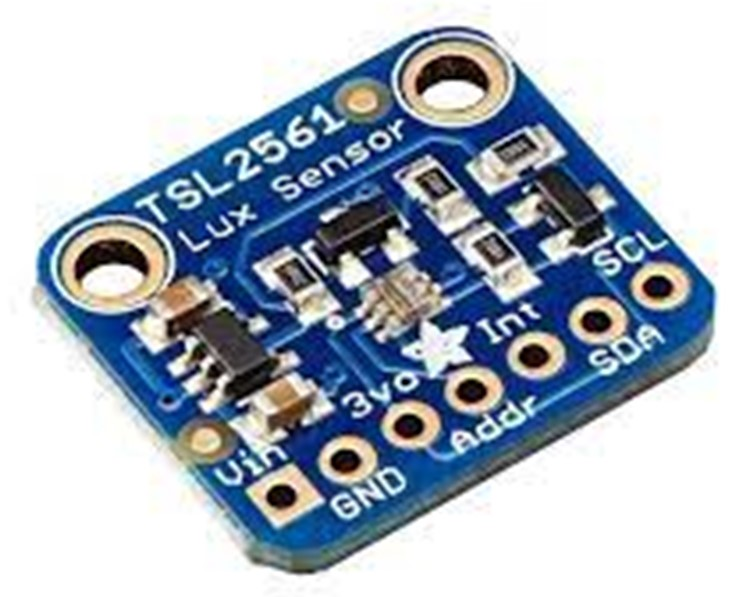
\includegraphics[width=0.4\textwidth]{\currfiledir/figures/TSL2561.jpg}
    \caption{TSL 2561}
    \cite{Light}
\end{figure}